\documentclass[11pt,a4paper]{article}
\usepackage[T1]{fontenc}
\usepackage{lmodern}
\usepackage{microtype}
\usepackage[margin=25mm,headheight=15pt]{geometry}
\usepackage{graphicx}
\usepackage{booktabs,tabularx,array}
\usepackage{amsmath,amssymb}
\usepackage{enumitem}
\usepackage{caption}
\usepackage{float}
\usepackage{fancyhdr}
\usepackage{tikz}
\usetikzlibrary{arrows.meta,positioning}
\usepackage[hidelinks]{hyperref}
\usepackage{url}
\setlength{\parindent}{0pt}
\setlength{\parskip}{5pt}
\setcounter{tocdepth}{1}
\setlength{\emergencystretch}{2em}
\setlist{nosep,leftmargin=1.5em}
\captionsetup{font=small,labelfont=bf}
\renewcommand{\arraystretch}{1.18}
\newcolumntype{Y}{>{\raggedright\arraybackslash}X}
\pagestyle{fancy}
\fancyhf{}
\fancyfoot[C]{\thepage}
\renewcommand{\headrulewidth}{0pt}
\hypersetup{pdftitle={Aegis: Emergency First-Response Coordination},pdfauthor={Ayush Pandey and Dheeraj Sutram},pdfsubject={Campus incident coordination prototype}}

\begin{document}
\hypersetup{pageanchor=false}
\begin{titlepage}
\centering
\vspace*{18mm}
{\large\scshape AI Innovate-A-Thon\par}
\vspace{6mm}
{\normalsize Topic 10\par}
\vspace{28mm}
{\fontsize{42}{48}\selectfont\bfseries Aegis\par}
\vspace{8mm}
{\LARGE Emergency First-Response\par Coordination\par}
\vspace{9mm}
{\large A campus event exercise prototype\par}
\vspace{14mm}
\rule{0.72\textwidth}{0.5pt}\par
\vspace{10mm}
{\large\scshape Project Report\par}
\vfill
\begin{tabular}{lr}
\textbf{Contributor} & \textbf{Registration number} \\
\addlinespace[3pt]
Ayush Pandey & 24BIT0394 \\
Dheeraj Sutram & 24BIT0416 \\
\end{tabular}
\vspace{20mm}

{\normalsize 24 October 2026\par}
\vspace*{10mm}
\end{titlepage}

\pagenumbering{roman}
\hypersetup{pageanchor=true}
\section*{Abstract}
Aegis is an incident coordination application for synthetic campus event exercises. It organises incoming text reports into provisional incident groups, displays the source evidence, suggests a priority using explicit rules, and records the coordinator's decisions. Reports are stored before analysis so incomplete inputs and model failures remain visible. The coordinator can confirm or reject a grouping, move reports, merge or split incidents, change priority, and review conflicting accounts.

The application uses Python, FastAPI and SQLite for analysis, API access and persistence, with a React and TypeScript interface. An optional local MiniLM encoder supports semantic matching. The measured build uses a deterministic lexical-hash fallback with location, time and category checks. On a fixed synthetic test set of 60 reports across 20 incident families, contextual lexical grouping achieved pairwise precision of 1.000, recall of 0.621 and F1 of 0.766. It produced zero false merge pairs and 25 missed pairs. All reports carried review flags in this mode. The implementation therefore supports inspectable grouping and correction while retaining substantial human review. Evaluation is limited to synthetic fixtures and does not establish suitability for live emergency operations.

\vspace{3mm}
\textbf{Keywords:} incident coordination, report grouping, human review, evidence retention, synthetic evaluation.

\vspace{5mm}
\tableofcontents
\clearpage
\pagenumbering{arabic}

\section{Introduction}
\subsection{Problem and intended user}
During a campus event, organisers may receive several accounts of the same situation. One person may identify a door, another may describe a queue, and a later report may say that access has been restored. A report stream leaves the coordinator to reconcile wording, location, timing and uncertainty while keeping track of separate incidents.

Aegis gives one coordinator a shared board for this work. Each incident contains the original reports, proposed membership, supporting comparisons, priority reasons and review history. The interface also shows reports with unknown locations and incomplete descriptions. The bundled map is a schematic of an illustrative event site.

\subsection{Objectives}
The project implements Topic 10 of the AI Innovate-A-Thon brief. Its objectives are to:
\begin{enumerate}
\item preserve every accepted report and its original text;
\item propose incident groups using text and event context;
\item expose the reasons behind grouping and priority suggestions;
\item retain conflicting and changing accounts for inspection;
\item support coordinator corrections with a persistent audit history; and
\item evaluate grouping and review behaviour on reproducible synthetic fixtures.
\end{enumerate}

The prototype accepts English text through a manual form and a controlled replay. All bundled people, reports and incident labels are synthetic. The application has no emergency service connection or responder dispatch function.

\subsection{Project contribution}
The contribution is the implemented coordination workflow: report preservation, contextual grouping, visible uncertainty, conflict inspection and reversible human decisions in one application. Sentence embeddings and cosine similarity are established methods. Sentence-BERT provides a basis for comparing sentence representations~\cite{sbert}, and the optional Aegis adapter uses an existing pretrained model. The project does not train a new encoder.

\section{Requirements and system design}
\subsection{Functional requirements}
Table~\ref{tab:requirements} relates the central requirements to their implemented behaviour. The system distinguishes an accepted report, a proposed incident membership and a coordinator decision. This distinction lets the board retain uncertainty without discarding the underlying account.

\begin{table}[H]
\centering\small
\caption{Core requirements and implementation}
\label{tab:requirements}
\begin{tabularx}{\textwidth}{@{}p{38mm}Y@{}}
\toprule
Requirement & Implemented behaviour \\
\midrule
Report intake & Validated text, optional zone, sublocation and event time, with an idempotency key. \\
Incident grouping & Incremental comparisons, context constraints, an anchor check and a candidate margin. \\
Visible evidence & Original text, component scores, missing fields and decision reasons. \\
Explicit priority & Versioned exercise rules with supporting source phrases. \\
Human correction & Confirm, reject, move, merge, split, priority override and status change. \\
History & Transactional updates with reasons, before/after values and event ownership. \\
Reproducible exercise & Step-controlled replay through the ordinary ingestion path. \\
\bottomrule
\end{tabularx}
\end{table}

\subsection{Architecture}
The Python backend contains the API, analysis engine, SQLite storage and evaluation pipeline. The frontend uses TanStack Start, React and TypeScript. Vite and Bun provide frontend development and build tooling. The interface uses shadcn components, Base UI primitives and self-hosted Figtree fonts.

\begin{figure}[H]
\centering
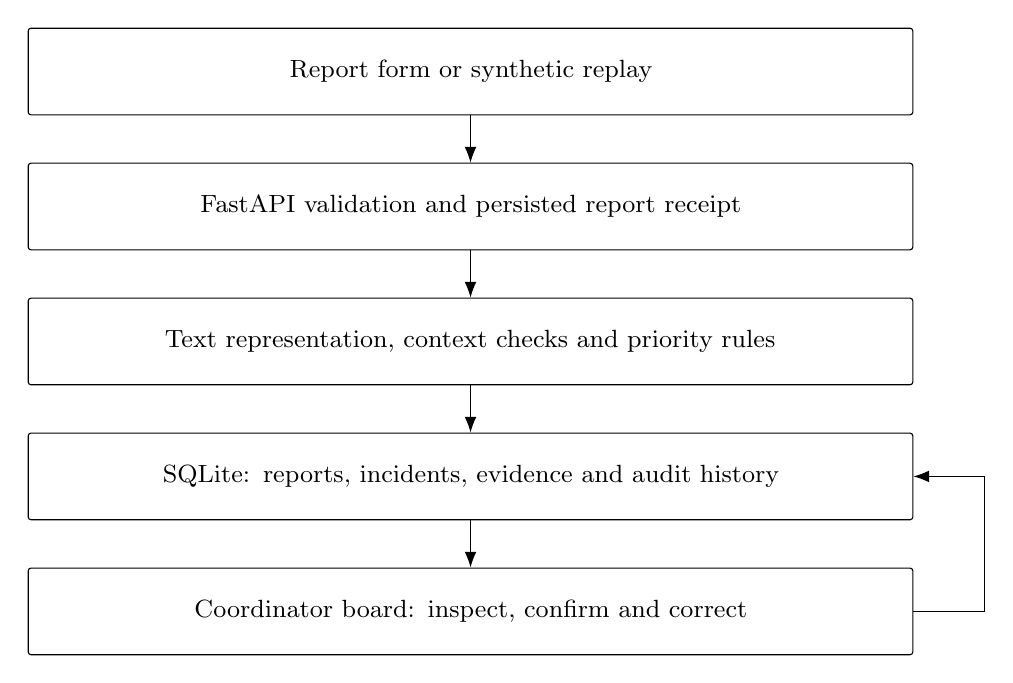
\begin{tikzpicture}[node distance=6mm,box/.style={draw,rounded corners=1pt,align=center,text width=110mm,minimum height=11mm,font=\small},flow/.style={-{Latex[length=2mm]},thin}]
\node[box] (input) {Report form or synthetic replay};
\node[box,below=of input] (receipt) {FastAPI validation and persisted report receipt};
\node[box,below=of receipt] (engine) {Text representation, context checks and priority rules};
\node[box,below=of engine] (store) {SQLite: reports, incidents, evidence and audit history};
\node[box,below=of store] (ui) {Coordinator board: inspect, confirm and correct};
\draw[flow] (input)--(receipt);
\draw[flow] (receipt)--(engine);
\draw[flow] (engine)--(store);
\draw[flow] (store)--(ui);
\draw[flow] (ui.east)--++(9mm,0)|-(store.east);
\end{tikzpicture}
\caption{Aegis processing and review flow. Coordinator changes return through the API and storage transaction.}
\label{fig:architecture}
\end{figure}

The frontend polls a snapshot endpoint and applies successful mutation responses. The backend exposes the active matching mode through its health endpoint. The application binds to the local host by default and uses a single SQLite database for the exercise state.

\subsection{Persistence and invariants}
An accepted report is committed with a provisional incident before analysis. Its original text is retained exactly. Analysis adds category, claims, a representation and review reasons. If analysis fails, the report remains accessible with a visible failure or review state.

The storage model separates events, reports, report analysis, incidents, memberships, matching evidence, conflicts, review decisions, rejection constraints, audit events and replay sessions. Each report has one current membership. Historical evidence keeps its original comparison while remaining accessible through the report's current group.

Idempotency is scoped to the event. Repeating a key with the same payload returns the existing receipt. Reusing it for a different payload returns a conflict. Coordinator mutations validate incident versions and commit state changes together with their audit entries. A new replay creates another event and preserves earlier history.

\section{Report analysis and grouping}
\subsection{Text representations}
The optional semantic adapter loads \texttt{all-MiniLM-L6-v2} from a local model cache. The model maps text to 384-dimensional vectors~\cite{minilm}. Sentence Transformers supports comparison of these representations using cosine similarity~\cite{sts}. Aegis normalises vectors and records the representation revision with each analysis.

When the optional package or weights are unavailable, or inference fails, the engine uses a deterministic 512-dimensional lexical-hash representation. It hashes token counts into a fixed vector and compares the resulting vectors. This mode relies on lexical overlap and can miss differently worded accounts. The dashboard and evaluation identify the fallback explicitly. MiniLM weights were unavailable in the measured environment, so the results in Section~\ref{sec:evaluation} describe lexical grouping.

\subsection{Context and candidate checks}
Candidate comparisons use the same exercise event. Location checks distinguish a broad zone from a specific shared sublocation or described entity. Time checks use compatible event timestamps, with a default window of 20 minutes and a 120-minute window for missing-person cases. Category and entity checks identify incompatible accounts. Unknown fields are recorded as missing.

Automatic attachment requires known compatible time and specific shared context. A conflict in location, time, category or entity can block attachment. The incoming report is checked against group members for incompatibilities. The first member acts as the anchor, and its text similarity must pass the active mode's minimum. This prevents a chain of individually similar reports from bypassing the anchor requirement.

\subsection{Ranking score}
For the available components, the pair score is
\begin{equation}
S(r_i,r_j)=\frac{\sum_{k\in A}w_k s_k(r_i,r_j)}{\sum_{k\in A}w_k},
\label{eq:score}
\end{equation}
where $A$ contains the available text, location, time and category components. Their weights are 0.65, 0.20, 0.10 and 0.05 respectively. With complete inputs, the denominator is one. Missing components are omitted for ranking, while required context gates still apply. The score is an uncalibrated ranking value.

An incident's candidate score is the mean of comparisons with up to its first four members. Table~\ref{tab:gates} gives the implemented attachment thresholds. The best eligible candidate must also exceed the runner-up by at least 0.08. Without a qualifying candidate, the incoming report remains in a separate reviewable group and may retain suggested matches.

\begin{table}[H]
\centering\small
\caption{Attachment thresholds in the current matching configuration}
\label{tab:gates}
\begin{tabularx}{\textwidth}{@{}Yrr@{}}
\toprule
Gate & MiniLM mode & Lexical mode \\
\midrule
Minimum candidate score & 0.82 & 0.33 \\
Minimum anchor text similarity & 0.62 & 0.05 \\
Minimum candidate margin & 0.08 & 0.08 \\
\bottomrule
\end{tabularx}
\end{table}

The lexical thresholds were developed using the development fixtures. Version 2 adds the 0.05 anchor requirement to prevent shared context alone from attaching textually unrelated reports. This choice makes the fallback conservative and leaves more same-family pairs for manual review.

\subsection{Decision procedure}
The ingestion and matching procedure is:
\begin{enumerate}
\item Validate the payload and event-scoped idempotency key.
\item Commit the original report and its provisional incident.
\item Extract supported claims, assign the exercise priority and create the text representation.
\item Compare eligible incident members and store the component evidence.
\item Reject incompatible candidates and coordinator-rejected pairings.
\item Apply the anchor, context, candidate score and margin gates.
\item Save the proposed membership, priority and review flags. Preserve a separate incident when the gates fail.
\end{enumerate}

Grouping remains provisional until the coordinator reviews it. A coordinator rejection adds a constraint so a later matching pass cannot silently recreate that pairing. Late analysis also preserves decisions made while the report was being processed.

\section{Priority, conflict and coordinator review}
\subsection{Exercise priority policy}
Priority is computed using explicit text rules and retained source phrases. Table~\ref{tab:priority} summarises the implemented labels. These labels organise a synthetic review queue and require human interpretation.

\begin{table}[H]
\centering\small
\caption{Exercise priority labels}
\label{tab:priority}
\begin{tabularx}{\textwidth}{@{}p{25mm}Y@{}}
\toprule
Label & Basis \\
\midrule
P0 & A supported affirmative phrase alleging immediate danger. \\
P1 & A blocked exit, a medical concern, or a missing-person report with a supported vulnerability cue. \\
P2 & A facility issue with a reporter-supplied zone. \\
Unassessed & Insufficient information or no supported affirmative policy rule. \\
\bottomrule
\end{tabularx}
\end{table}

Rules account for supported negations and hypothetical language. Equipment terms such as ``fire extinguisher'' and ``smoke machine'' are excluded from the corresponding standalone danger trigger. These checks cover a finite English vocabulary. The incident assessment retains the strongest unresolved priority signal across its reports.

\subsection{Conflicting and changing accounts}
Claim extraction retains a field, value and original supporting phrase. Opposing values can produce a conflict entry with the relevant report identifiers and source spans. An exit described as blocked and later described as clear remains inspectable as a changing or conflicting account. The system cannot establish which account is true from report volume alone.

A later reassuring report does not automatically close the incident or cancel unresolved urgent evidence. The coordinator can resolve or reopen the conflict with a reason. Conflict counts refer to opposing report pairs, so several pairs can arise within one incident.

\subsection{Coordinator actions and audit}
The coordinator can confirm selected membership, reject a pairing, move reports, merge incidents or split selected reports into a new group. Priority, workflow status and conflict review have separate actions. Each mutation requires a reason and the version of every affected incident that the coordinator reviewed.

A stale request receives an HTTP 409 response. The coordinator must inspect the changed state before rebasing the action. Grouping changes update memberships, evidence access, conflict state and rejection constraints within a transaction. Audit records contain the actor, action, affected identifiers, reason, before/after values and timestamp. This is an application audit history with ordinary database administration limits.

\section{User interface and demonstration}
The Operations screen combines incident counts, the queue, an illustrative map and the selected incident inspector. Priority labels accompany colour. Unknown-location reports remain in a visible tray, and keyboard users can select map markers. The New report page accepts fresh synthetic wording with optional location and event time.

The replay advances one fixture at a time through the ordinary intake API. It does not pass expected incident labels to the matcher. The demo sequence includes duplicate accounts, an incomplete singleton, changing Exit A accounts and a coordinator correction.

The main workflow is to start a fresh replay, advance the reports, select an incident, inspect source text and evidence, then confirm or correct its membership. The Evaluation page shows the measured method, grouping metrics, explicit checks and limitations. Earlier event history remains available when another exercise begins.

\begin{figure}[H]
\centering
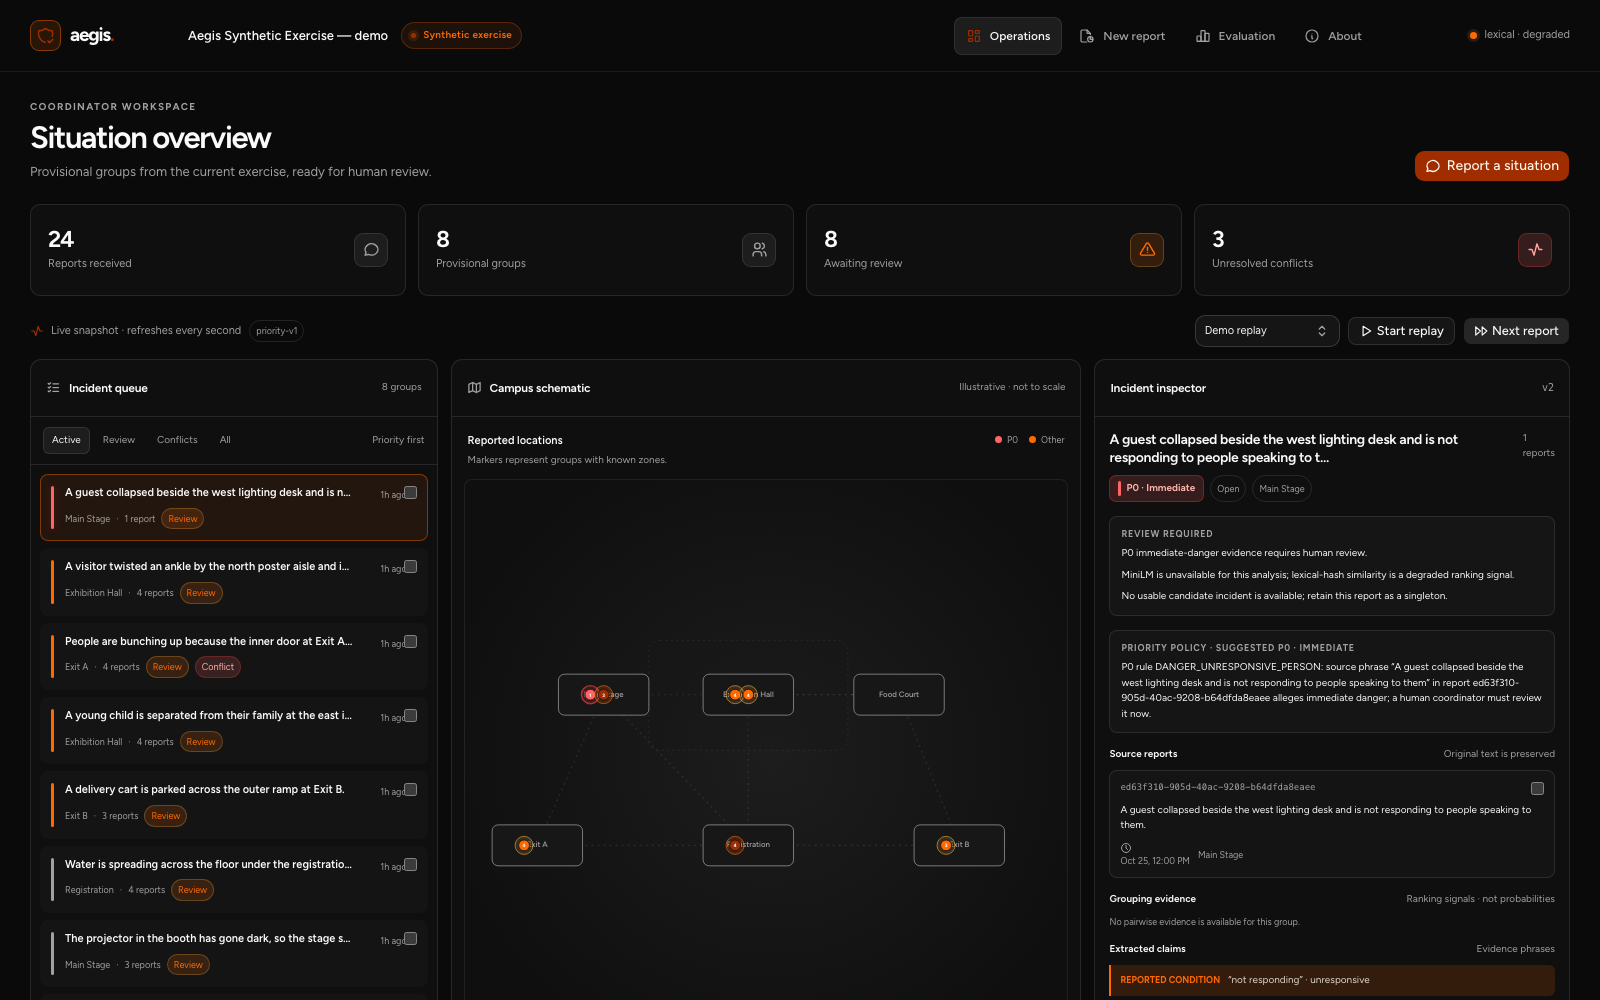
\includegraphics[width=\textwidth]{screenshots/dashboard-wide.png}
\caption{Operations after the 24-report demo replay. The board shows eight provisional groups and the active lexical matching mode.}
\label{fig:dashboard}
\end{figure}

\begin{figure}[H]
\centering
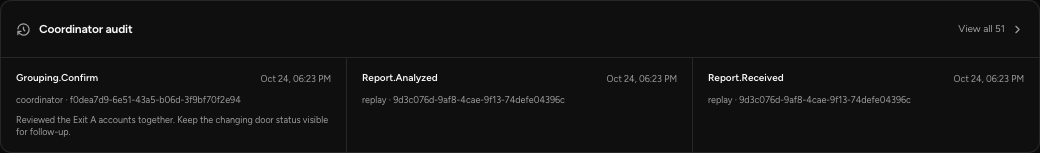
\includegraphics[width=\textwidth]{screenshots/audit.png}
\caption{Audit entries after a coordinator confirms selected membership and records a reason.}
\label{fig:audit}
\end{figure}

\section{Evaluation}
\label{sec:evaluation}
\subsection{Dataset and protocol}
The versioned fixtures contain 144 reports across three sets, as shown in Table~\ref{tab:data}. Runtime inputs and ground-truth labels are stored separately. The evaluator reads the fixed test inputs and labels, and the matcher receives only report content and context.

\begin{table}[H]
\centering\small
\caption{Synthetic fixtures used by the project}
\label{tab:data}
\begin{tabularx}{\textwidth}{@{}lrrY@{}}
\toprule
Set & Reports & Families & Purpose \\
\midrule
Demo & 24 & 8 & Step-controlled demonstration \\
Development & 60 & 20 & Threshold and configuration development \\
Test/regression & 60 & 20 & Fixed grouping and policy measurements \\
\bottomrule
\end{tabularx}
\end{table}

Categories and scenario patterns recur across sets. Test cases were inspected during engineering, and discovered failures became regression cases. These measurements describe a small synthetic regression benchmark. They cannot establish accuracy across independent events, languages or operational conditions.

\subsection{Metrics and baseline}
Grouping is evaluated over unordered report pairs. A true positive ($TP$) is a same-family pair placed together. A false positive ($FP$) is a different-family pair placed together, counted as a false merge pair. A false negative ($FN$) is a same-family pair left apart, counted as a missed pair. The metrics are
\begin{equation}
P=\frac{TP}{TP+FP},\qquad R=\frac{TP}{TP+FN},\qquad
F_1=\frac{2PR}{P+R}.
\end{equation}
The review rate is the fraction of reports carrying a review reason. Its interpretation depends on the method's flagging rules.

The baseline uses token-set Jaccard similarity with simple zone and time gates. It is compared with Aegis contextual lexical grouping on the same inputs. The baseline's limited review flags do not establish that the remaining reports were safe to accept.

\subsection{Measured grouping results}
Table~\ref{tab:results} reproduces the saved executable measurement in \path{evaluation/results/latest.json}, generated on 24 October 2026. No semantic encoder result is available for this environment.

\begin{table}[H]
\centering\small
\caption{Pairwise results on the 60-report test/regression set}
\label{tab:results}
\begin{tabularx}{\textwidth}{@{}Yrr@{}}
\toprule
Measure & Jaccard baseline & Aegis lexical \\
\midrule
Precision & 1.000 & 1.000 \\
Recall & 0.061 & 0.621 \\
F1 & 0.114 & 0.766 \\
False merge pairs & 0 & 0 \\
Missed pairs & 62 & 25 \\
Reports flagged for review & 8.3\% & 100\% \\
\bottomrule
\end{tabularx}
\end{table}

The label set contains 66 same-family pairs. The baseline recovers four and Aegis recovers 41. Aegis therefore finds 37 additional same-family pairs while maintaining zero observed false merge pairs on this fixture. Its 25 missed pairs and 100\% review rate show the remaining grouping and review workload. Perfect observed precision on this small set is limited evidence about future inputs.

The saved run measured median analysis-plus-incremental-grouping latency of 11.843\,ms and a 95th percentile of 22.564\,ms. These are process-local evaluator timings for this hardware and workload. They exclude an end-to-end browser response-time study.

\subsection{Policy and retention checks}
All six explicit evaluator checks passed: retention of all 60 reports, expected fixture cardinality, the explicit P0 case, the negative priority control, visibility of the changing-report case, and reviewability of the incomplete case. The last four checks each contain one labelled case or group, which limits the breadth of this evidence.

The separate API replay retained 24 reports in eight provisional groups, exposed three opposing report-pair conflicts and recorded 50 audit entries before an additional coordinator correction. The conflict count describes evidence pairs. It does not count independently verified events.

\section{Implementation verification}
The project verification record dated 24 October 2026 reports 196 passing backend tests and 140 passing frontend tests. Table~\ref{tab:verification} lists the recorded coverage totals. The backend scope includes the application and fixture generator. The frontend scope includes all source modules, component primitives and generated route registration.

\begin{table}[H]
\centering\small
\caption{Recorded verification results}
\label{tab:verification}
\begin{tabularx}{\textwidth}{@{}Yrr@{}}
\toprule
Measure & Executed / total & Coverage \\
\midrule
Backend statements & 2,414 / 2,414 & 100\% \\
Backend branches & 844 / 844 & 100\% \\
Frontend statements & 834 / 834 & 100\% \\
Frontend branches & 565 / 565 & 100\% \\
Frontend functions & 245 / 245 & 100\% \\
Frontend lines & 745 / 745 & 100\% \\
\bottomrule
\end{tabularx}
\end{table}

Tests cover malformed payloads, exact source retention, idempotency conflicts, event isolation, analysis failure, grouping corrections, stale versions and concurrency races. Five integration tests execute the frontend's grouping payload builder with Bun and submit its output to FastAPI for confirm, reject, move, merge and split.

The recorded verification also includes Ruff lint and formatting, strict TypeScript checks, client and server production builds, and a Chromium smoke test against both services. The browser test advances all 24 replay reports, submits fresh text, confirms membership, inspects the audit and opens evaluation. Coverage measures execution of the included code paths. It leaves correctness for untested input distributions and operational conditions unresolved.

The API validates the Host header, checks browser origins for mutations, requires JSON POST bodies and returns non-caching responses. Production authentication remains future work. SQLite transactions and version checks address consistency within the prototype's local exercise model.

\section{Limitations and further work}
\subsection{Current limits}
The measured matcher depends on lexical overlap and a small set of English extraction rules. Paraphrases, unsupported negations, ambiguous references and unseen descriptions can affect grouping or priority. Optional semantic inference is implemented but remains unmeasured with actual MiniLM weights in the recorded environment.

The synthetic fixtures are small and share recurring categories and scenario structures. No independent deployment study measured coordinator workload, response time, injuries or other safety outcomes. The map is illustrative. The application assumes a single coordinator and local use, with no authenticated user roles or production operating policy.

\subsection{Further work}
The next evaluation should run the cached MiniLM model and lexical fallback on a larger independently prepared set. Useful additions include varied paraphrases, multilingual inputs, explicit temporal changes, challenging negative controls and error analysis by incident type. Thresholds should be fixed before the independent evaluation.

Interface evaluation should observe coordinators completing realistic exercises and measure correction effort, missed information and decision time. Access control, operational security review, backups, deployment monitoring and accessibility testing on real devices are required before broader use. Any operational priority policy would need approval from the responsible stakeholders.

The intended sustainability link is SDG 11 through coordination during community events, with secondary relevance to SDG 3. These are intended areas of relevance. The project has measured software behaviour and synthetic grouping outcomes.

\section{Conclusion}
Aegis implements a complete local workflow for receiving synthetic reports, proposing incident groups, inspecting evidence and recording coordinator corrections. Its persistence model keeps source accounts accessible through uncertainty, conflicts and analysis failure. The contextual lexical method recovers more same-family pairs than the Jaccard baseline on the fixed test set, while retaining every report for review. The current evidence supports the prototype's inspectable coordination workflow and defines the evaluation needed for further development.

\begingroup\small\raggedright
\begin{thebibliography}{9}
\bibitem{sbert} N. Reimers and I. Gurevych, ``Sentence-BERT: Sentence Embeddings using Siamese BERT-Networks,'' EMNLP-IJCNLP, 2019. \href{https://arxiv.org/abs/1908.10084}{arXiv:1908.10084}.
\bibitem{minilm} Sentence Transformers, ``all-MiniLM-L6-v2.'' \href{https://huggingface.co/sentence-transformers/all-MiniLM-L6-v2}{Hugging Face model card}. Accessed 24 October 2026.
\bibitem{sts} Sentence Transformers, ``Semantic Textual Similarity.'' \href{https://sbert.net/docs/sentence_transformer/usage/semantic_textual_similarity.html}{Sentence Transformers documentation}. Accessed 24 October 2026.
\bibitem{project} Aegis project repository, implementation and verification materials, 24 October 2026. \path{backend/aegis/}, \path{frontend/src/}, \path{docs/API_CONTRACT.md}, \path{docs/VERIFICATION.md}, \path{evaluation/results/latest.json} and \path{evaluation/results/verification.json}.
\end{thebibliography}
\endgroup
\end{document}
